% Options for packages loaded elsewhere
% Options for packages loaded elsewhere
\PassOptionsToPackage{unicode}{hyperref}
\PassOptionsToPackage{hyphens}{url}
\PassOptionsToPackage{dvipsnames,svgnames,x11names}{xcolor}
%
\documentclass[
  11pt,
  a4paper,
  onecolumn]{article}
\usepackage{xcolor}
\usepackage[top=1in,left=1in,right=1in,bottom=1in]{geometry}
\usepackage{amsmath,amssymb}
\setcounter{secnumdepth}{-\maxdimen} % remove section numbering
\usepackage{iftex}
\ifPDFTeX
  \usepackage[T1]{fontenc}
  \usepackage[utf8]{inputenc}
  \usepackage{textcomp} % provide euro and other symbols
\else % if luatex or xetex
  \usepackage{unicode-math} % this also loads fontspec
  \defaultfontfeatures{Scale=MatchLowercase}
  \defaultfontfeatures[\rmfamily]{Ligatures=TeX,Scale=1}
\fi
\usepackage{lmodern}
\ifPDFTeX\else
  % xetex/luatex font selection
\fi
% Use upquote if available, for straight quotes in verbatim environments
\IfFileExists{upquote.sty}{\usepackage{upquote}}{}
\IfFileExists{microtype.sty}{% use microtype if available
  \usepackage[]{microtype}
  \UseMicrotypeSet[protrusion]{basicmath} % disable protrusion for tt fonts
}{}
\usepackage{setspace}
\makeatletter
\@ifundefined{KOMAClassName}{% if non-KOMA class
  \IfFileExists{parskip.sty}{%
    \usepackage{parskip}
  }{% else
    \setlength{\parindent}{0pt}
    \setlength{\parskip}{6pt plus 2pt minus 1pt}}
}{% if KOMA class
  \KOMAoptions{parskip=half}}
\makeatother
% Make \paragraph and \subparagraph free-standing
\makeatletter
\ifx\paragraph\undefined\else
  \let\oldparagraph\paragraph
  \renewcommand{\paragraph}{
    \@ifstar
      \xxxParagraphStar
      \xxxParagraphNoStar
  }
  \newcommand{\xxxParagraphStar}[1]{\oldparagraph*{#1}\mbox{}}
  \newcommand{\xxxParagraphNoStar}[1]{\oldparagraph{#1}\mbox{}}
\fi
\ifx\subparagraph\undefined\else
  \let\oldsubparagraph\subparagraph
  \renewcommand{\subparagraph}{
    \@ifstar
      \xxxSubParagraphStar
      \xxxSubParagraphNoStar
  }
  \newcommand{\xxxSubParagraphStar}[1]{\oldsubparagraph*{#1}\mbox{}}
  \newcommand{\xxxSubParagraphNoStar}[1]{\oldsubparagraph{#1}\mbox{}}
\fi
\makeatother

\usepackage{color}
\usepackage{fancyvrb}
\newcommand{\VerbBar}{|}
\newcommand{\VERB}{\Verb[commandchars=\\\{\}]}
\DefineVerbatimEnvironment{Highlighting}{Verbatim}{commandchars=\\\{\}}
% Add ',fontsize=\small' for more characters per line
\newenvironment{Shaded}{}{}
\newcommand{\AlertTok}[1]{\textcolor[rgb]{1.00,0.33,0.33}{\textbf{#1}}}
\newcommand{\AnnotationTok}[1]{\textcolor[rgb]{0.42,0.45,0.49}{#1}}
\newcommand{\AttributeTok}[1]{\textcolor[rgb]{0.84,0.23,0.29}{#1}}
\newcommand{\BaseNTok}[1]{\textcolor[rgb]{0.00,0.36,0.77}{#1}}
\newcommand{\BuiltInTok}[1]{\textcolor[rgb]{0.84,0.23,0.29}{#1}}
\newcommand{\CharTok}[1]{\textcolor[rgb]{0.01,0.18,0.38}{#1}}
\newcommand{\CommentTok}[1]{\textcolor[rgb]{0.42,0.45,0.49}{#1}}
\newcommand{\CommentVarTok}[1]{\textcolor[rgb]{0.42,0.45,0.49}{#1}}
\newcommand{\ConstantTok}[1]{\textcolor[rgb]{0.00,0.36,0.77}{#1}}
\newcommand{\ControlFlowTok}[1]{\textcolor[rgb]{0.84,0.23,0.29}{#1}}
\newcommand{\DataTypeTok}[1]{\textcolor[rgb]{0.84,0.23,0.29}{#1}}
\newcommand{\DecValTok}[1]{\textcolor[rgb]{0.00,0.36,0.77}{#1}}
\newcommand{\DocumentationTok}[1]{\textcolor[rgb]{0.42,0.45,0.49}{#1}}
\newcommand{\ErrorTok}[1]{\textcolor[rgb]{1.00,0.33,0.33}{\underline{#1}}}
\newcommand{\ExtensionTok}[1]{\textcolor[rgb]{0.84,0.23,0.29}{\textbf{#1}}}
\newcommand{\FloatTok}[1]{\textcolor[rgb]{0.00,0.36,0.77}{#1}}
\newcommand{\FunctionTok}[1]{\textcolor[rgb]{0.44,0.26,0.76}{#1}}
\newcommand{\ImportTok}[1]{\textcolor[rgb]{0.01,0.18,0.38}{#1}}
\newcommand{\InformationTok}[1]{\textcolor[rgb]{0.42,0.45,0.49}{#1}}
\newcommand{\KeywordTok}[1]{\textcolor[rgb]{0.84,0.23,0.29}{#1}}
\newcommand{\NormalTok}[1]{\textcolor[rgb]{0.14,0.16,0.18}{#1}}
\newcommand{\OperatorTok}[1]{\textcolor[rgb]{0.14,0.16,0.18}{#1}}
\newcommand{\OtherTok}[1]{\textcolor[rgb]{0.44,0.26,0.76}{#1}}
\newcommand{\PreprocessorTok}[1]{\textcolor[rgb]{0.84,0.23,0.29}{#1}}
\newcommand{\RegionMarkerTok}[1]{\textcolor[rgb]{0.42,0.45,0.49}{#1}}
\newcommand{\SpecialCharTok}[1]{\textcolor[rgb]{0.00,0.36,0.77}{#1}}
\newcommand{\SpecialStringTok}[1]{\textcolor[rgb]{0.01,0.18,0.38}{#1}}
\newcommand{\StringTok}[1]{\textcolor[rgb]{0.01,0.18,0.38}{#1}}
\newcommand{\VariableTok}[1]{\textcolor[rgb]{0.89,0.38,0.04}{#1}}
\newcommand{\VerbatimStringTok}[1]{\textcolor[rgb]{0.01,0.18,0.38}{#1}}
\newcommand{\WarningTok}[1]{\textcolor[rgb]{1.00,0.33,0.33}{#1}}

\usepackage{longtable,booktabs,array}
\usepackage{calc} % for calculating minipage widths
% Correct order of tables after \paragraph or \subparagraph
\usepackage{etoolbox}
\makeatletter
\patchcmd\longtable{\par}{\if@noskipsec\mbox{}\fi\par}{}{}
\makeatother
% Allow footnotes in longtable head/foot
\IfFileExists{footnotehyper.sty}{\usepackage{footnotehyper}}{\usepackage{footnote}}
\makesavenoteenv{longtable}
\usepackage{graphicx}
\makeatletter
\newsavebox\pandoc@box
\newcommand*\pandocbounded[1]{% scales image to fit in text height/width
  \sbox\pandoc@box{#1}%
  \Gscale@div\@tempa{\textheight}{\dimexpr\ht\pandoc@box+\dp\pandoc@box\relax}%
  \Gscale@div\@tempb{\linewidth}{\wd\pandoc@box}%
  \ifdim\@tempb\p@<\@tempa\p@\let\@tempa\@tempb\fi% select the smaller of both
  \ifdim\@tempa\p@<\p@\scalebox{\@tempa}{\usebox\pandoc@box}%
  \else\usebox{\pandoc@box}%
  \fi%
}
% Set default figure placement to htbp
\def\fps@figure{htbp}
\makeatother





\setlength{\emergencystretch}{3em} % prevent overfull lines

\providecommand{\tightlist}{%
  \setlength{\itemsep}{0pt}\setlength{\parskip}{0pt}}



 


\makeatletter
\@ifpackageloaded{caption}{}{\usepackage{caption}}
\AtBeginDocument{%
\ifdefined\contentsname
  \renewcommand*\contentsname{Table of contents}
\else
  \newcommand\contentsname{Table of contents}
\fi
\ifdefined\listfigurename
  \renewcommand*\listfigurename{List of Figures}
\else
  \newcommand\listfigurename{List of Figures}
\fi
\ifdefined\listtablename
  \renewcommand*\listtablename{List of Tables}
\else
  \newcommand\listtablename{List of Tables}
\fi
\ifdefined\figurename
  \renewcommand*\figurename{Figure}
\else
  \newcommand\figurename{Figure}
\fi
\ifdefined\tablename
  \renewcommand*\tablename{Table}
\else
  \newcommand\tablename{Table}
\fi
}
\@ifpackageloaded{float}{}{\usepackage{float}}
\floatstyle{ruled}
\@ifundefined{c@chapter}{\newfloat{codelisting}{h}{lop}}{\newfloat{codelisting}{h}{lop}[chapter]}
\floatname{codelisting}{Listing}
\newcommand*\listoflistings{\listof{codelisting}{List of Listings}}
\makeatother
\makeatletter
\makeatother
\makeatletter
\@ifpackageloaded{caption}{}{\usepackage{caption}}
\@ifpackageloaded{subcaption}{}{\usepackage{subcaption}}
\makeatother
\usepackage{bookmark}
\IfFileExists{xurl.sty}{\usepackage{xurl}}{} % add URL line breaks if available
\urlstyle{same}
\hypersetup{
  pdftitle={Static PID-5 and ESI},
  pdfauthor={Corrado Caudek},
  colorlinks=true,
  linkcolor={blue},
  filecolor={Maroon},
  citecolor={Blue},
  urlcolor={Blue},
  pdfcreator={LaTeX via pandoc}}


\title{Static PID-5 and ESI}
\author{Corrado Caudek}
\date{}
\begin{document}
\maketitle


\setstretch{1}
Le misure ``basali'' corrispondenti al questionario ESI.

\begin{Shaded}
\begin{Highlighting}[]
\CommentTok{\# Read and process \textquotesingle{}esi\_bf\textquotesingle{} data}
\NormalTok{esi\_bf }\OtherTok{\textless{}{-}}\NormalTok{ rio}\SpecialCharTok{::}\FunctionTok{import}\NormalTok{(}
\NormalTok{  here}\SpecialCharTok{::}\FunctionTok{here}\NormalTok{(}
    \StringTok{"data"}\NormalTok{,}
    \StringTok{"processed"}\NormalTok{,}
    \StringTok{"esi\_bf.csv"}
\NormalTok{  )}
\NormalTok{) }\SpecialCharTok{|\textgreater{}}
\NormalTok{  dplyr}\SpecialCharTok{::}\FunctionTok{distinct}\NormalTok{(user\_id, }\AttributeTok{.keep\_all =} \ConstantTok{TRUE}\NormalTok{) }\SpecialCharTok{|\textgreater{}} \CommentTok{\# Keep only distinct user\_id}
\NormalTok{  dplyr}\SpecialCharTok{::}\FunctionTok{select}\NormalTok{(user\_id, esi\_bf) }\CommentTok{\# Select relevant columns}
\end{Highlighting}
\end{Shaded}

\begin{Shaded}
\begin{Highlighting}[]
\CommentTok{\# Read and process \textquotesingle{}pid5\textquotesingle{} data}
\NormalTok{pid5 }\OtherTok{\textless{}{-}}\NormalTok{ rio}\SpecialCharTok{::}\FunctionTok{import}\NormalTok{(}
\NormalTok{  here}\SpecialCharTok{::}\FunctionTok{here}\NormalTok{(}
    \StringTok{"data"}\NormalTok{,}
    \StringTok{"processed"}\NormalTok{,}
    \StringTok{"pid5.csv"}
\NormalTok{  )}
\NormalTok{) }\SpecialCharTok{|\textgreater{}}
\NormalTok{  dplyr}\SpecialCharTok{::}\FunctionTok{distinct}\NormalTok{(user\_id, }\AttributeTok{.keep\_all =} \ConstantTok{TRUE}\NormalTok{) }\SpecialCharTok{|\textgreater{}}  \CommentTok{\# Keep only distinct user\_id}
\NormalTok{  dplyr}\SpecialCharTok{::}\FunctionTok{select}\NormalTok{(user\_id, }\FunctionTok{starts\_with}\NormalTok{(}\StringTok{"domain\_"}\NormalTok{)) }\CommentTok{\# Select domain variables}

\CommentTok{\# Merge \textquotesingle{}esi\_bf\textquotesingle{} and \textquotesingle{}pid5\textquotesingle{} data by user\_id}
\NormalTok{df }\OtherTok{\textless{}{-}} \FunctionTok{left\_join}\NormalTok{(esi\_bf, pid5, }\AttributeTok{by =} \StringTok{"user\_id"}\NormalTok{)}
\end{Highlighting}
\end{Shaded}

\begin{Shaded}
\begin{Highlighting}[]
\CommentTok{\# Define list of user IDs with careless responding}
\NormalTok{user\_id\_with\_careless\_responding }\OtherTok{\textless{}{-}} \FunctionTok{c}\NormalTok{(}
  \StringTok{"ma\_se\_2005\_11\_14\_490"}\NormalTok{,}
  \StringTok{"reve20041021036"}\NormalTok{,}
  \StringTok{"di\_ma\_2005\_10\_20\_756"}\NormalTok{,}
  \StringTok{"pa\_sc\_2005\_09\_10\_468"}\NormalTok{,}
  \StringTok{"il\_re\_2006\_01\_18\_645"}\NormalTok{,}
  \StringTok{"so\_ma\_2003\_10\_13\_804"}\NormalTok{,}
  \StringTok{"lo\_ca\_2005\_05\_07\_05\_437"}\NormalTok{,}
  \StringTok{"va\_ma\_2005\_05\_31\_567"}\NormalTok{,}
  \StringTok{"no\_un\_2005\_06\_29\_880"}\NormalTok{,}
  \StringTok{"an\_bo\_1988\_08\_24\_166"}\NormalTok{,}
  \StringTok{"st\_ma\_2004\_04\_21\_426"}\NormalTok{,}
  \StringTok{"an\_st\_2005\_10\_16\_052"}\NormalTok{,}
  \StringTok{"vi\_de\_2002\_12\_30\_067"}\NormalTok{,}
  \StringTok{"gi\_ru\_2005\_03\_08\_033"}\NormalTok{,}
  \StringTok{"al\_mi\_2005\_03\_05\_844"}\NormalTok{,}
  \StringTok{"la\_ma\_2006\_01\_31\_787"}\NormalTok{,}
  \StringTok{"gi\_lo\_2004\_06\_27\_237"}\NormalTok{,}
  \StringTok{"ch\_bi\_2001\_01\_28\_407"}\NormalTok{,}
  \StringTok{"al\_pe\_2001\_04\_20\_079"}\NormalTok{,}
  \StringTok{"le\_de\_2003\_09\_05\_067"}\NormalTok{,}
  \StringTok{"fe\_gr\_2002\_02\_19\_434"}\NormalTok{,}
  \StringTok{"ma\_ba\_2002\_09\_09\_052"}\NormalTok{,}
  \StringTok{"ca\_gi\_2003\_09\_16\_737"}\NormalTok{,}
  \StringTok{"an\_to\_2003\_08\_06\_114"}\NormalTok{,}
  \StringTok{"al\_se\_2003\_07\_28\_277"}\NormalTok{,}
  \StringTok{"ja\_tr\_2002\_10\_06\_487"}\NormalTok{,}
  \StringTok{"el\_ci\_2002\_02\_15\_057"}\NormalTok{,}
  \StringTok{"se\_ti\_2000\_03\_04\_975"}\NormalTok{,}
  \StringTok{"co\_ga\_2003\_10\_29\_614"}\NormalTok{,}
  \StringTok{"al\_ba\_2003\_18\_07\_905"}\NormalTok{,}
  \StringTok{"bi\_ro\_2003\_09\_07\_934"}\NormalTok{,}
  \StringTok{"an\_va\_2004\_04\_08\_527"}\NormalTok{,}
  \StringTok{"ev\_cr\_2003\_01\_27\_573"}
\NormalTok{)}

\CommentTok{\# Filter out users with careless responses}
\NormalTok{df1 }\OtherTok{\textless{}{-}}\NormalTok{ df[}\SpecialCharTok{!}\NormalTok{(df}\SpecialCharTok{$}\NormalTok{user\_id }\SpecialCharTok{\%in\%}\NormalTok{ user\_id\_with\_careless\_responding), ]}
\end{Highlighting}
\end{Shaded}

\begin{Shaded}
\begin{Highlighting}[]
\CommentTok{\# Read EMA data and rename \textquotesingle{}subj\_code\textquotesingle{} to \textquotesingle{}user\_id\textquotesingle{}}
\NormalTok{ema\_raw }\OtherTok{\textless{}{-}} \FunctionTok{readRDS}\NormalTok{(}
\NormalTok{  here}\SpecialCharTok{::}\FunctionTok{here}\NormalTok{(}
    \StringTok{"data"}\NormalTok{,}
    \StringTok{"raw"}\NormalTok{,}
    \StringTok{"ema"}\NormalTok{,}
    \StringTok{"ema\_data\_scoring.RDS"}
\NormalTok{  )}
\NormalTok{) }\SpecialCharTok{|\textgreater{}}
\NormalTok{  dplyr}\SpecialCharTok{::}\FunctionTok{rename}\NormalTok{(}
    \AttributeTok{user\_id =}\NormalTok{ subj\_code}
\NormalTok{  )}

\CommentTok{\# Merge EMA data with filtered main data}
\NormalTok{df2 }\OtherTok{\textless{}{-}} \FunctionTok{left\_join}\NormalTok{(df1, ema\_raw, }\AttributeTok{by =} \StringTok{"user\_id"}\NormalTok{)}

\CommentTok{\# Verify number of unique users}
\FunctionTok{length}\NormalTok{(}\FunctionTok{unique}\NormalTok{(df2}\SpecialCharTok{$}\NormalTok{user\_id))}
\end{Highlighting}
\end{Shaded}

\begin{verbatim}
[1] 429
\end{verbatim}

\subsection{Compliance}\label{compliance}

Escludiamo i soggetti che hanno risposto a meno di 10 notifiche.

\begin{Shaded}
\begin{Highlighting}[]
\CommentTok{\# Conta quante risposte EMA ha fornito ciascun soggetto}
\NormalTok{user\_counts }\OtherTok{\textless{}{-}}\NormalTok{ df2 }\SpecialCharTok{\%\textgreater{}\%}
  \FunctionTok{group\_by}\NormalTok{(user\_id) }\SpecialCharTok{\%\textgreater{}\%}
  \FunctionTok{summarise}\NormalTok{(}\AttributeTok{n\_responses =} \FunctionTok{n}\NormalTok{()) }\SpecialCharTok{\%\textgreater{}\%}
  \FunctionTok{ungroup}\NormalTok{()}

\CommentTok{\# Tieni solo i soggetti con almeno 10 risposte}
\NormalTok{valid\_users }\OtherTok{\textless{}{-}}\NormalTok{ user\_counts }\SpecialCharTok{\%\textgreater{}\%}
  \FunctionTok{filter}\NormalTok{(n\_responses }\SpecialCharTok{\textgreater{}=} \DecValTok{10}\NormalTok{) }\SpecialCharTok{\%\textgreater{}\%}
  \FunctionTok{pull}\NormalTok{(user\_id)}

\CommentTok{\# Filtra il dataframe originale}
\NormalTok{df2 }\OtherTok{\textless{}{-}}\NormalTok{ df2 }\SpecialCharTok{\%\textgreater{}\%}
\NormalTok{  dplyr}\SpecialCharTok{::}\FunctionTok{filter}\NormalTok{(user\_id }\SpecialCharTok{\%in\%}\NormalTok{ valid\_users)}
\end{Highlighting}
\end{Shaded}

\begin{Shaded}
\begin{Highlighting}[]
\FunctionTok{length}\NormalTok{(}\FunctionTok{unique}\NormalTok{(df2}\SpecialCharTok{$}\NormalTok{user\_id))}
\end{Highlighting}
\end{Shaded}

\begin{verbatim}
[1] 379
\end{verbatim}

\subsection{Generate negative instant
mood}\label{generate-negative-instant-mood}

\begin{Shaded}
\begin{Highlighting}[]
\CommentTok{\# Costruisce una misura media dell\textquotesingle{}affetto negativo momentaneo}

\CommentTok{\# Seleziona solo le colonne rilevanti (per velocità)}
\NormalTok{items }\OtherTok{\textless{}{-}} \FunctionTok{c}\NormalTok{(}\StringTok{"sad"}\NormalTok{, }\StringTok{"angry"}\NormalTok{, }\StringTok{"happy"}\NormalTok{, }\StringTok{"satisfied"}\NormalTok{)}

\CommentTok{\# Imputa i missing (1 solo imputazione, dato che i NA sono pochi)}
\NormalTok{imputed }\OtherTok{\textless{}{-}} \FunctionTok{mice}\NormalTok{(df2[, items], }\AttributeTok{m =} \DecValTok{1}\NormalTok{, }\AttributeTok{maxit =} \DecValTok{10}\NormalTok{, }\AttributeTok{seed =} \DecValTok{123}\NormalTok{)}
\end{Highlighting}
\end{Shaded}

\begin{verbatim}

 iter imp variable
  1   1  sad  angry  happy  satisfied
  2   1  sad  angry  happy  satisfied
  3   1  sad  angry  happy  satisfied
  4   1  sad  angry  happy  satisfied
  5   1  sad  angry  happy  satisfied
  6   1  sad  angry  happy  satisfied
  7   1  sad  angry  happy  satisfied
  8   1  sad  angry  happy  satisfied
  9   1  sad  angry  happy  satisfied
  10   1  sad  angry  happy  satisfied
\end{verbatim}

\begin{Shaded}
\begin{Highlighting}[]
\CommentTok{\# Estrai il dataset imputato e sostituisci le colonne originali}
\NormalTok{df2\_imputed }\OtherTok{\textless{}{-}} \FunctionTok{complete}\NormalTok{(imputed)}
\NormalTok{df2[, items] }\OtherTok{\textless{}{-}}\NormalTok{ df2\_imputed[, items]}

\NormalTok{df2 }\OtherTok{\textless{}{-}}\NormalTok{ df2 }\SpecialCharTok{\%\textgreater{}\%}
  \FunctionTok{mutate}\NormalTok{(}
    \AttributeTok{happy\_reversed =} \DecValTok{100} \SpecialCharTok{{-}}\NormalTok{ happy, }\CommentTok{\# Scala 0{-}100}
    \AttributeTok{satisfied\_reversed =} \DecValTok{100} \SpecialCharTok{{-}}\NormalTok{ satisfied,}
    \AttributeTok{neg\_aff\_ema =} \FunctionTok{rowMeans}\NormalTok{(}
      \FunctionTok{cbind}\NormalTok{(sad, angry, happy\_reversed, satisfied\_reversed),}
      \AttributeTok{na.rm =} \ConstantTok{TRUE}
\NormalTok{    )}
\NormalTok{  )}
\end{Highlighting}
\end{Shaded}

\begin{Shaded}
\begin{Highlighting}[]
\NormalTok{df3 }\OtherTok{\textless{}{-}}\NormalTok{ df2 }\SpecialCharTok{\%\textgreater{}\%}
\NormalTok{  dplyr}\SpecialCharTok{::}\FunctionTok{select}\NormalTok{(}
\NormalTok{    user\_id, }
\NormalTok{    esi\_bf,}
\NormalTok{    neg\_aff\_ema, }
    \FunctionTok{starts\_with}\NormalTok{(}\StringTok{"domain\_"}\NormalTok{),}
\NormalTok{    pid5\_negative\_affectivity, pid5\_detachment, pid5\_antagonism, }
\NormalTok{    pid5\_disinhibition, pid5\_psychoticism }
\NormalTok{  )}
\end{Highlighting}
\end{Shaded}

\begin{Shaded}
\begin{Highlighting}[]
\NormalTok{df4 }\OtherTok{\textless{}{-}}\NormalTok{ df3[}\SpecialCharTok{!}\FunctionTok{is.na}\NormalTok{(df3}\SpecialCharTok{$}\NormalTok{domain\_negative\_affect), ]}
\FunctionTok{length}\NormalTok{(}\FunctionTok{unique}\NormalTok{(df4}\SpecialCharTok{$}\NormalTok{user\_id))}
\end{Highlighting}
\end{Shaded}

\begin{verbatim}
[1] 350
\end{verbatim}

\begin{Shaded}
\begin{Highlighting}[]
\CommentTok{\# Imputa i missing (1 solo imputazione, dato che i NA sono pochi)}
\NormalTok{imputed }\OtherTok{\textless{}{-}} \FunctionTok{mice}\NormalTok{(df4, }\AttributeTok{m =} \DecValTok{1}\NormalTok{, }\AttributeTok{maxit =} \DecValTok{10}\NormalTok{, }\AttributeTok{seed =} \DecValTok{123}\NormalTok{)}
\end{Highlighting}
\end{Shaded}

\begin{verbatim}

 iter imp variable
  1   1  pid5_negative_affectivity  pid5_detachment  pid5_antagonism  pid5_disinhibition  pid5_psychoticism
  2   1  pid5_negative_affectivity  pid5_detachment  pid5_antagonism  pid5_disinhibition  pid5_psychoticism
  3   1  pid5_negative_affectivity  pid5_detachment  pid5_antagonism  pid5_disinhibition  pid5_psychoticism
  4   1  pid5_negative_affectivity  pid5_detachment  pid5_antagonism  pid5_disinhibition  pid5_psychoticism
  5   1  pid5_negative_affectivity  pid5_detachment  pid5_antagonism  pid5_disinhibition  pid5_psychoticism
  6   1  pid5_negative_affectivity  pid5_detachment  pid5_antagonism  pid5_disinhibition  pid5_psychoticism
  7   1  pid5_negative_affectivity  pid5_detachment  pid5_antagonism  pid5_disinhibition  pid5_psychoticism
  8   1  pid5_negative_affectivity  pid5_detachment  pid5_antagonism  pid5_disinhibition  pid5_psychoticism
  9   1  pid5_negative_affectivity  pid5_detachment  pid5_antagonism  pid5_disinhibition  pid5_psychoticism
  10   1  pid5_negative_affectivity  pid5_detachment  pid5_antagonism  pid5_disinhibition  pid5_psychoticism
\end{verbatim}

\begin{verbatim}
Warning: Number of logged events: 1
\end{verbatim}

\begin{Shaded}
\begin{Highlighting}[]
\CommentTok{\# Estrai il dataset imputato e sostituisci le colonne originali}
\NormalTok{df5 }\OtherTok{\textless{}{-}} \FunctionTok{complete}\NormalTok{(imputed)}
\end{Highlighting}
\end{Shaded}

\begin{Shaded}
\begin{Highlighting}[]
\NormalTok{df5\_scaled }\OtherTok{\textless{}{-}}\NormalTok{ df5 }\SpecialCharTok{\%\textgreater{}\%}
\NormalTok{  dplyr}\SpecialCharTok{::}\FunctionTok{mutate}\NormalTok{(}
    \CommentTok{\# Applica la standardizzazione (scale) a tutte le colonne selezionate}
    \CommentTok{\# tranne user\_id. as.vector() è usato per assicurare che l\textquotesingle{}output sia un vettore.}
\NormalTok{    dplyr}\SpecialCharTok{::}\FunctionTok{across}\NormalTok{(}
      \FunctionTok{c}\NormalTok{(}
\NormalTok{        esi\_bf,}
\NormalTok{        neg\_aff\_ema, }
\NormalTok{        domain\_negative\_affect,   }
\NormalTok{        domain\_detachment,}
\NormalTok{        domain\_antagonism,}
\NormalTok{        domain\_disinhibition,}
\NormalTok{        domain\_psychoticism,}
\NormalTok{        pid5\_negative\_affectivity,}
\NormalTok{        pid5\_detachment,}
\NormalTok{        pid5\_antagonism,}
\NormalTok{        pid5\_disinhibition,}
\NormalTok{        pid5\_psychoticism}
\NormalTok{      ),}
      \SpecialCharTok{\textasciitilde{}} \FunctionTok{as.vector}\NormalTok{(}\FunctionTok{scale}\NormalTok{(.))}
\NormalTok{    )}
\NormalTok{  )}
\end{Highlighting}
\end{Shaded}

Nel caso presente:

esi\_bf è costante entro ogni user\_id. Le variabili come neg\_aff\_ema
e le pid5\_ sono tempo-varianti. La variabile esi\_bf è costante nel
tempo per ciascun soggetto, quindi non è possibile usare dati a livello
momentaneo (EMA) per predire variazione intra-soggettiva che non esiste
nell'outcome.

Il modo corretto di affrontare la domanda di ricerca, preservando la
validità statistica del confronto, è:

\begin{itemize}
\tightlist
\item
  Aggregare le variabili EMA (come neg\_aff\_ema,
  pid5\_negative\_affectivity, ecc.) a livello del soggetto.
\item
  Usare media per il confronto.
\end{itemize}

Costruiamo dunque due modelli alternativi a livello soggetto:

\begin{itemize}
\tightlist
\item
  model\_base\_subject: senza interazioni,
\item
  model\_alt\_subject: con le interazioni (tra tratti stabili e tratti
  EMA aggregati).
\end{itemize}

\begin{Shaded}
\begin{Highlighting}[]
\NormalTok{df\_subject }\OtherTok{\textless{}{-}}\NormalTok{ df5\_scaled }\SpecialCharTok{\%\textgreater{}\%}
  \FunctionTok{group\_by}\NormalTok{(user\_id) }\SpecialCharTok{\%\textgreater{}\%}
  \FunctionTok{summarise}\NormalTok{(}
    \AttributeTok{esi\_bf =} \FunctionTok{first}\NormalTok{(esi\_bf),}
    \AttributeTok{neg\_aff\_ema\_m =} \FunctionTok{mean}\NormalTok{(neg\_aff\_ema, }\AttributeTok{na.rm =} \ConstantTok{TRUE}\NormalTok{),}
    \AttributeTok{pid5\_neg\_aff\_m =} \FunctionTok{mean}\NormalTok{(pid5\_negative\_affectivity, }\AttributeTok{na.rm =} \ConstantTok{TRUE}\NormalTok{),}
    \AttributeTok{pid5\_detach\_m =} \FunctionTok{mean}\NormalTok{(pid5\_detachment, }\AttributeTok{na.rm =} \ConstantTok{TRUE}\NormalTok{),}
    \AttributeTok{pid5\_antag\_m =} \FunctionTok{mean}\NormalTok{(pid5\_antagonism, }\AttributeTok{na.rm =} \ConstantTok{TRUE}\NormalTok{),}
    \AttributeTok{pid5\_disin\_m =} \FunctionTok{mean}\NormalTok{(pid5\_disinhibition, }\AttributeTok{na.rm =} \ConstantTok{TRUE}\NormalTok{),}
    \AttributeTok{pid5\_psych\_m =} \FunctionTok{mean}\NormalTok{(pid5\_psychoticism, }\AttributeTok{na.rm =} \ConstantTok{TRUE}\NormalTok{),}
    \AttributeTok{domain\_negative\_affect =} \FunctionTok{first}\NormalTok{(domain\_negative\_affect),}
    \AttributeTok{domain\_detachment =} \FunctionTok{first}\NormalTok{(domain\_detachment),}
    \AttributeTok{domain\_antagonism =} \FunctionTok{first}\NormalTok{(domain\_antagonism),}
    \AttributeTok{domain\_disinhibition =} \FunctionTok{first}\NormalTok{(domain\_disinhibition),}
    \AttributeTok{domain\_psychoticism =} \FunctionTok{first}\NormalTok{(domain\_psychoticism)}
\NormalTok{  )}
\end{Highlighting}
\end{Shaded}

\begin{Shaded}
\begin{Highlighting}[]
\NormalTok{model\_base }\OtherTok{\textless{}{-}} \FunctionTok{brm}\NormalTok{(}
\NormalTok{  esi\_bf }\SpecialCharTok{\textasciitilde{}} \DecValTok{1} \SpecialCharTok{+} 
\NormalTok{    domain\_negative\_affect }\SpecialCharTok{+}\NormalTok{ domain\_detachment }\SpecialCharTok{+}
\NormalTok{    domain\_antagonism }\SpecialCharTok{+}\NormalTok{ domain\_disinhibition }\SpecialCharTok{+}\NormalTok{ domain\_psychoticism,}
  \AttributeTok{data =}\NormalTok{ df\_subject,}
  \AttributeTok{family =} \FunctionTok{asym\_laplace}\NormalTok{(),}
  \AttributeTok{prior =} \FunctionTok{c}\NormalTok{(}
    \FunctionTok{prior}\NormalTok{(}\FunctionTok{normal}\NormalTok{(}\DecValTok{0}\NormalTok{, }\DecValTok{1}\NormalTok{), }\AttributeTok{class =} \StringTok{"Intercept"}\NormalTok{),}
    \FunctionTok{prior}\NormalTok{(}\FunctionTok{normal}\NormalTok{(}\DecValTok{0}\NormalTok{, }\DecValTok{1}\NormalTok{), }\AttributeTok{class =} \StringTok{"b"}\NormalTok{),}
    \FunctionTok{prior}\NormalTok{(}\FunctionTok{exponential}\NormalTok{(}\DecValTok{1}\NormalTok{), }\AttributeTok{class =} \StringTok{"sigma"}\NormalTok{)}
\NormalTok{  ),}
  \AttributeTok{chains =} \DecValTok{4}\NormalTok{,}
  \AttributeTok{cores =} \DecValTok{4}\NormalTok{,}
  \AttributeTok{iter =} \DecValTok{2000}\NormalTok{,}
  \AttributeTok{seed =} \DecValTok{123}\NormalTok{,}
  \AttributeTok{backend =} \StringTok{"cmdstanr"}\NormalTok{,}
  \CommentTok{\# algorithm = "meanfield",}
  \AttributeTok{save\_pars =} \FunctionTok{save\_pars}\NormalTok{(}\AttributeTok{all =} \ConstantTok{TRUE}\NormalTok{)}
\NormalTok{)}
\end{Highlighting}
\end{Shaded}

\begin{Shaded}
\begin{Highlighting}[]
\CommentTok{\# Posterior predictive check for the baseline model}
\FunctionTok{pp\_check}\NormalTok{(model\_base)}
\end{Highlighting}
\end{Shaded}

\begin{verbatim}
Using 10 posterior draws for ppc type 'dens_overlay' by default.
\end{verbatim}

\pandocbounded{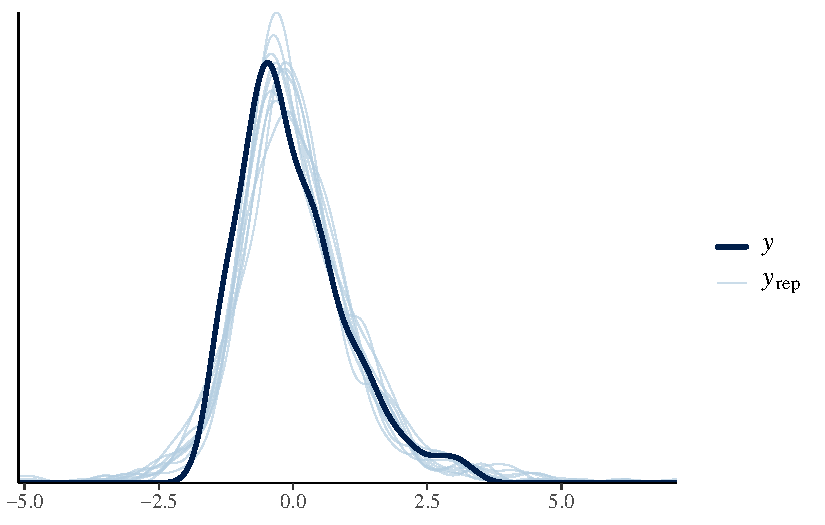
\includegraphics[keepaspectratio]{pid5_esi_files/figure-pdf/unnamed-chunk-15-1.pdf}}

\begin{Shaded}
\begin{Highlighting}[]
\FunctionTok{print}\NormalTok{(model\_base)}
\end{Highlighting}
\end{Shaded}

\begin{verbatim}
 Family: asym_laplace 
  Links: mu = identity; sigma = identity; quantile = identity 
Formula: esi_bf ~ 1 + domain_negative_affect + domain_detachment + domain_antagonism + domain_disinhibition + domain_psychoticism 
   Data: df_subject (Number of observations: 350) 
  Draws: 4 chains, each with iter = 2000; warmup = 1000; thin = 1;
         total post-warmup draws = 4000

Regression Coefficients:
                       Estimate Est.Error l-95% CI u-95% CI Rhat Bulk_ESS
Intercept                 -0.34      0.09    -0.52    -0.17 1.00     1798
domain_negative_affect    -0.13      0.06    -0.23    -0.02 1.00     2165
domain_detachment         -0.10      0.05    -0.21     0.00 1.00     2476
domain_antagonism          0.07      0.05    -0.03     0.18 1.00     2863
domain_disinhibition       0.25      0.06     0.13     0.37 1.00     2377
domain_psychoticism        0.17      0.07     0.04     0.31 1.00     2271
                       Tail_ESS
Intercept                  1618
domain_negative_affect     2484
domain_detachment          2921
domain_antagonism          2694
domain_disinhibition       2612
domain_psychoticism        2084

Further Distributional Parameters:
         Estimate Est.Error l-95% CI u-95% CI Rhat Bulk_ESS Tail_ESS
sigma        0.33      0.02     0.29     0.37 1.00     2285     2487
quantile     0.38      0.04     0.31     0.45 1.00     1745     1809

Draws were sampled using sample(hmc). For each parameter, Bulk_ESS
and Tail_ESS are effective sample size measures, and Rhat is the potential
scale reduction factor on split chains (at convergence, Rhat = 1).
\end{verbatim}

\begin{Shaded}
\begin{Highlighting}[]
\NormalTok{model\_alt }\OtherTok{\textless{}{-}} \FunctionTok{brm}\NormalTok{(}
\NormalTok{  esi\_bf }\SpecialCharTok{\textasciitilde{}} \DecValTok{1} \SpecialCharTok{+}
\NormalTok{    domain\_negative\_affect }\SpecialCharTok{*}\NormalTok{ pid5\_neg\_aff\_m }\SpecialCharTok{+}
\NormalTok{    domain\_detachment }\SpecialCharTok{*}\NormalTok{ pid5\_detach\_m }\SpecialCharTok{+}
\NormalTok{    domain\_antagonism }\SpecialCharTok{*}\NormalTok{ pid5\_antag\_m }\SpecialCharTok{+}
\NormalTok{    domain\_disinhibition }\SpecialCharTok{*}\NormalTok{ pid5\_disin\_m }\SpecialCharTok{+}
\NormalTok{    domain\_psychoticism }\SpecialCharTok{*}\NormalTok{ pid5\_psych\_m,}
  \AttributeTok{data =}\NormalTok{ df\_subject,}
  \AttributeTok{family =} \FunctionTok{asym\_laplace}\NormalTok{(),}
  \AttributeTok{prior =} \FunctionTok{c}\NormalTok{(}
    \FunctionTok{prior}\NormalTok{(}\FunctionTok{normal}\NormalTok{(}\DecValTok{0}\NormalTok{, }\DecValTok{1}\NormalTok{), }\AttributeTok{class =} \StringTok{"Intercept"}\NormalTok{),}
    \FunctionTok{prior}\NormalTok{(}\FunctionTok{normal}\NormalTok{(}\DecValTok{0}\NormalTok{, }\DecValTok{1}\NormalTok{), }\AttributeTok{class =} \StringTok{"b"}\NormalTok{),}
    \FunctionTok{prior}\NormalTok{(}\FunctionTok{exponential}\NormalTok{(}\DecValTok{1}\NormalTok{), }\AttributeTok{class =} \StringTok{"sigma"}\NormalTok{)}
\NormalTok{  ),}
  \AttributeTok{chains =} \DecValTok{4}\NormalTok{,}
  \AttributeTok{cores =} \DecValTok{4}\NormalTok{,}
  \AttributeTok{iter =} \DecValTok{2000}\NormalTok{,}
  \AttributeTok{seed =} \DecValTok{123}\NormalTok{,}
  \AttributeTok{backend =} \StringTok{"cmdstanr"}\NormalTok{,}
  \CommentTok{\# algorithm = "meanfield",}
  \AttributeTok{save\_pars =} \FunctionTok{save\_pars}\NormalTok{(}\AttributeTok{all =} \ConstantTok{TRUE}\NormalTok{)}
\NormalTok{)}
\end{Highlighting}
\end{Shaded}

\begin{Shaded}
\begin{Highlighting}[]
\FunctionTok{pp\_check}\NormalTok{(model\_alt)}
\end{Highlighting}
\end{Shaded}

\begin{verbatim}
Using 10 posterior draws for ppc type 'dens_overlay' by default.
\end{verbatim}

\pandocbounded{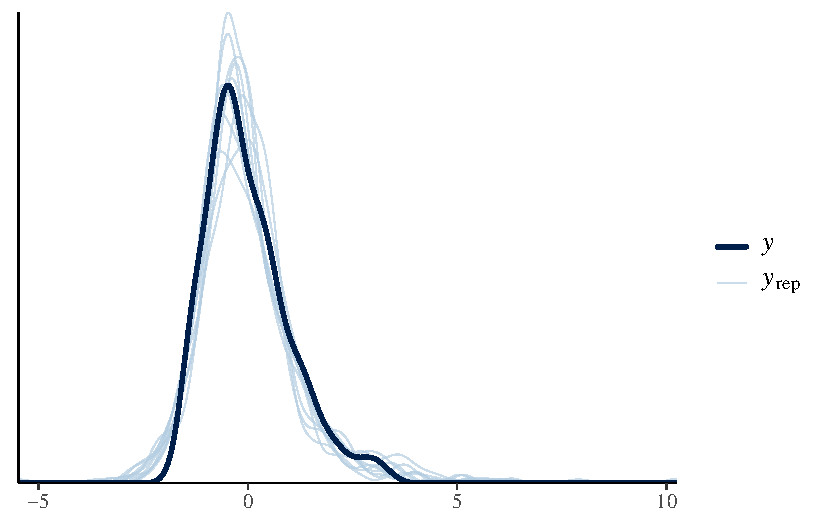
\includegraphics[keepaspectratio]{pid5_esi_files/figure-pdf/unnamed-chunk-18-1.pdf}}

\begin{Shaded}
\begin{Highlighting}[]
\FunctionTok{print}\NormalTok{(model\_alt)}
\end{Highlighting}
\end{Shaded}

\begin{verbatim}
 Family: asym_laplace 
  Links: mu = identity; sigma = identity; quantile = identity 
Formula: esi_bf ~ 1 + domain_negative_affect * pid5_neg_aff_m + domain_detachment * pid5_detach_m + domain_antagonism * pid5_antag_m + domain_disinhibition * pid5_disin_m + domain_psychoticism * pid5_psych_m 
   Data: df_subject (Number of observations: 350) 
  Draws: 4 chains, each with iter = 2000; warmup = 1000; thin = 1;
         total post-warmup draws = 4000

Regression Coefficients:
                                      Estimate Est.Error l-95% CI u-95% CI Rhat
Intercept                                -0.48      0.13    -0.73    -0.24 1.00
domain_negative_affect                   -0.05      0.07    -0.19     0.08 1.00
pid5_neg_aff_m                           -0.11      0.09    -0.28     0.06 1.00
domain_detachment                        -0.12      0.05    -0.23    -0.01 1.00
pid5_detach_m                             0.14      0.08    -0.03     0.30 1.00
domain_antagonism                         0.04      0.06    -0.07     0.16 1.00
pid5_antag_m                             -0.01      0.09    -0.20     0.17 1.00
domain_disinhibition                      0.22      0.07     0.09     0.35 1.00
pid5_disin_m                             -0.03      0.10    -0.23     0.17 1.00
domain_psychoticism                       0.18      0.07     0.04     0.31 1.00
pid5_psych_m                             -0.04      0.13    -0.28     0.21 1.00
domain_negative_affect:pid5_neg_aff_m     0.02      0.07    -0.12     0.14 1.00
domain_detachment:pid5_detach_m          -0.07      0.05    -0.16     0.04 1.00
domain_antagonism:pid5_antag_m            0.17      0.08     0.03     0.32 1.00
domain_disinhibition:pid5_disin_m        -0.00      0.08    -0.16     0.16 1.00
domain_psychoticism:pid5_psych_m         -0.07      0.07    -0.21     0.07 1.00
                                      Bulk_ESS Tail_ESS
Intercept                                 1184     1863
domain_negative_affect                    2016     2433
pid5_neg_aff_m                            2132     2583
domain_detachment                         2579     2527
pid5_detach_m                             2863     2189
domain_antagonism                         2521     2748
pid5_antag_m                              1892     2301
domain_disinhibition                      2601     2486
pid5_disin_m                              2592     2305
domain_psychoticism                       3039     2978
pid5_psych_m                              1849     2813
domain_negative_affect:pid5_neg_aff_m     2811     2499
domain_detachment:pid5_detach_m           2979     2433
domain_antagonism:pid5_antag_m            2785     2518
domain_disinhibition:pid5_disin_m         2249     2662
domain_psychoticism:pid5_psych_m          1911     2829

Further Distributional Parameters:
         Estimate Est.Error l-95% CI u-95% CI Rhat Bulk_ESS Tail_ESS
sigma        0.31      0.03     0.25     0.36 1.00     1339     1753
quantile     0.33      0.05     0.24     0.42 1.00     1097     1537

Draws were sampled using sample(hmc). For each parameter, Bulk_ESS
and Tail_ESS are effective sample size measures, and Rhat is the potential
scale reduction factor on split chains (at convergence, Rhat = 1).
\end{verbatim}

\begin{Shaded}
\begin{Highlighting}[]
\NormalTok{loo0 }\OtherTok{\textless{}{-}} \FunctionTok{loo}\NormalTok{(model\_base, }\AttributeTok{save\_psis =} \ConstantTok{TRUE}\NormalTok{)}
\NormalTok{loo1 }\OtherTok{\textless{}{-}} \FunctionTok{loo}\NormalTok{(model\_alt, }\AttributeTok{save\_psis =} \ConstantTok{TRUE}\NormalTok{)}
\FunctionTok{loo\_compare}\NormalTok{(loo0, loo1)}
\end{Highlighting}
\end{Shaded}

\begin{verbatim}
           elpd_diff se_diff
model_base  0.0       0.0   
model_alt  -7.7       4.6   
\end{verbatim}

\begin{Shaded}
\begin{Highlighting}[]
\FunctionTok{bayes\_R2}\NormalTok{(model\_base)}
\end{Highlighting}
\end{Shaded}

\begin{verbatim}
    Estimate  Est.Error       Q2.5     Q97.5
R2 0.1189947 0.03102776 0.05999484 0.1809222
\end{verbatim}

\begin{Shaded}
\begin{Highlighting}[]
\FunctionTok{bayes\_R2}\NormalTok{(model\_alt)}
\end{Highlighting}
\end{Shaded}

\begin{verbatim}
    Estimate  Est.Error       Q2.5     Q97.5
R2 0.1471981 0.03022991 0.08722664 0.2049597
\end{verbatim}

\subsection{Discussione dei risultati}\label{discussione-dei-risultati}

\subsubsection{Obiettivo dell'analisi}\label{obiettivo-dellanalisi}

L'obiettivo di questa analisi era verificare se le \textbf{dimensioni di
personalità patologica} misurate tramite il \textbf{PID-5} (in
particolare, le cinque dimensioni di dominio) siano in grado di predire
i punteggi individuali al composito \textbf{ESI\_BF}, che rappresenta un
indice di funzionamento adattivo o disfunzionale clinicamente rilevante.
Poiché \texttt{esi\_bf} è una misura stabile a livello individuale, sono
stati esclusi dal modello tutti i predittori momentanei, concentrandosi
esclusivamente su tratti stabili e su eventuali interazioni tra
\textbf{dimensioni stabili} e \textbf{variabili EMA aggregate} a livello
soggetto.

\subsubsection{Modello base}\label{modello-base}

Nel \textbf{modello base}, sono state considerate come predittori solo
le \textbf{cinque dimensioni del PID-5}:

\begin{itemize}
\tightlist
\item
  Negative Affect
\item
  Detachment
\item
  Antagonism
\item
  Disinhibition
\item
  Psychoticism
\end{itemize}

I risultati indicano che:

\begin{itemize}
\tightlist
\item
  \textbf{Negative Affect} (\(\beta\) = -0.13, CI95\% = {[}-0.23,
  -0.02{]}) e \textbf{Detachment} (\(\beta\) = -0.10, CI95\% = {[}-0.21,
  0.00{]}) sono \textbf{negativamente associati} al punteggio ESI\_BF.
  Ciò suggerisce che soggetti con maggiore affettività negativa o
  tendenza all'isolamento riferiscono livelli inferiori di funzionamento
  adattivo.
\item
  \textbf{Disinhibition} (\(\beta\) = 0.25, CI95\% = {[}0.13, 0.37{]}) e
  \textbf{Psychoticism} (\(\beta\) = 0.17, CI95\% = {[}0.04, 0.31{]})
  mostrano invece una \textbf{relazione positiva} con ESI\_BF. Questo
  risultato può apparire controintuitivo, ma potrebbe indicare che in
  alcuni contesti la disinibizione e tratti eccentrici siano collegati a
  strategie più attive di risposta o a bias di autovalutazione più
  positivi.
\end{itemize}

Il coefficiente di determinazione bayesiano (\textbf{Bayes R²}) è pari a
\textbf{0.12}, indicando che il modello spiega circa il \textbf{12\%
della varianza} interindividuale del punteggio ESI\_BF.

\subsubsection{Modello alternativo}\label{modello-alternativo}

Il \textbf{modello alternativo} ha aggiunto, per ciascun dominio del
PID-5, un'interazione con la \textbf{controparte EMA aggregata} (ad
esempio: \texttt{domain\_antagonism\ ×\ pid5\_antag\_m}), allo scopo di
esplorare se l'effetto dei tratti stabili cambia in funzione delle
fluttuazioni medie momentanee rilevate tramite EMA.

L'unico effetto chiaramente interpretabile nel modello alternativo è
l'interazione:

\begin{itemize}
\tightlist
\item
  \textbf{Domain Antagonism × EMA Antagonism} (\(\beta\) = 0.17, CI95\%
  = {[}0.03, 0.32{]})
\end{itemize}

Questo risultato suggerisce che per i soggetti con livelli elevati sia
di antagonismo stabile sia di antagonismo momentaneo, il punteggio
ESI\_BF tende ad aumentare. Potrebbe trattarsi di un sottogruppo di
individui che, pur presentando tratti interpersonali problematici,
mantengono una percezione soggettiva di sé come funzionanti (o
resilienti), oppure di un artefatto dovuto a risposte difensive o
sovracompensatorie.

Gli altri effetti principali e interazioni \textbf{non mostrano
associazioni robuste}, con intervalli di credibilità che comprendono lo
zero.

Il Bayes R² del modello alternativo è pari a \textbf{0.15}, un
incremento modesto rispetto al modello base.

\subsubsection{Confronto tra i modelli}\label{confronto-tra-i-modelli}

Per confrontare i due modelli è stato utilizzato il criterio
\textbf{LOO} (Leave-One-Out cross-validation), che stima la capacità
predittiva fuori campione. I risultati sono:

\begin{longtable}[]{@{}lll@{}}
\toprule\noalign{}
Modello & elpd\_diff & se\_diff \\
\midrule\noalign{}
\endhead
\bottomrule\noalign{}
\endlastfoot
Modello base & 0.0 & 0.0 \\
Modello alternativo & -7.7 & 4.6 \\
\end{longtable}

L'aggiunta delle interazioni con le medie EMA non ha migliorato le
prestazioni predittive: anzi, il modello alternativo presenta un ELPD
inferiore, con un'incertezza che non permette di concludere con
sicurezza che sia peggiore, ma suggerisce \textbf{nessun vantaggio
sostanziale} rispetto al modello più parsimonioso.

\subsubsection{Conclusioni}\label{conclusioni}

In sintesi:

\begin{itemize}
\tightlist
\item
  Le \textbf{dimensioni stabili del PID-5} spiegano una quota moderata
  della varianza nei punteggi ESI\_BF.
\item
  L'inclusione delle \textbf{interazioni con le misure EMA aggregate}
  non fornisce un guadagno informativo significativo e comporta un
  aumento della complessità del modello.
\item
  Il \textbf{modello base risulta preferibile}: è più semplice, offre
  interpretazioni più robuste e ha prestazioni predittive comparabili (o
  superiori) rispetto al modello esteso.
\end{itemize}

Questi risultati indicano che, per l'esito considerato, le
\textbf{caratteristiche stabili della personalità} sono i predittori più
rilevanti, e le fluttuazioni momentanee aggregate non sembrano
aggiungere informazioni predittive rilevanti \textbf{a livello
interindividuale}.




\end{document}
